\documentclass[]{article}

\usepackage{graphicx} % Allows including images
\usepackage{booktabs} % Allows the use of \toprule, \midrule and \bottomrule in tables
\usepackage{pdfpages}
\usepackage[percent]{overpic}
\usepackage[labelfont=bf]{caption}
\usepackage{amsmath}
\usepackage{amsfonts}
\usepackage{amssymb}
\usepackage[framemethod=TikZ]{mdframed}
\usepackage{tikz}

\usetikzlibrary{calc,trees,positioning,arrows,chains,shapes.geometric,%
	decorations.pathreplacing,decorations.pathmorphing,shapes,%
	matrix,shapes.symbols}

\tikzset{
	>=stealth',
	punktchain/.style={
		rectangle, 
		rounded corners, 
		% fill=black!10,
		draw=black, very thick,
		text width=10em, 
		minimum height=3em, 
		text centered, 
		on chain},
	line/.style={draw, thick, <-},
	element/.style={
		tape,
		top color=white,
		bottom color=blue!50!black!60!,
		minimum width=8em,
		draw=blue!40!black!90, very thick,
		text width=10em, 
		minimum height=3.5em, 
		text centered, 
		on chain},
	every join/.style={->, thick,shorten >=1pt},
	decoration={brace},
	tuborg/.style={decorate},
	tubnode/.style={midway, right=2pt},
}

\newcommand*\circled[1]{\tikz[baseline=(char.base)]{\node[shape=circle,draw,inner sep=2pt] (char) {#1};}}

%% Setting box counter
\newcounter{infobox}[section]
\renewcommand{\theinfobox}{\thesection.\arabic{infobox}}

%% Infobox style
\newenvironment{infobox}[1][]{%
    \refstepcounter{infobox}
    \begin{mdframed}[%
        frametitle={Box \theinfobox\ #1},
        skipabove=\baselineskip plus 2pt minus 1pt,
        skipbelow=\baselineskip plus 2pt minus 1pt,
        frametitleaboveskip= 7pt,
        frametitlebelowskip= 7pt,
        linewidth=0pt,
        linecolor=black,
        frametitlerule=false,
        frametitlebackgroundcolor=teal!30, % blue!10
        backgroundcolor=teal!30, % blue!10
        roundcorner=7pt,
    ]
}{
    \end{mdframed}
}	

%opening
\title{Enumeration and analysis of a small molecule universe}
\author{Stefan O. Gugler}

\begin{document}

\maketitle

\begin{abstract}
\input{abstract.tex}
\end{abstract}

%\section{Enumeration}
\label{sec:enum}
\subsection{Introduction and Specifications}
Even though our chemical space is truncated to the first and second coordination shell, which allows us to use a maximum of two heavy atoms, $e \in \{C,N,O,P,S\} $ per ligand, it is still enormously big. In a first step we assemble the ligands and in a second step we attach them combinatorially to a metal center to produce octahedral complexes. 

For the ligand design, a number of parameters are introduced to later impose constraints on them to further decrease the vastness of the space. These parameters include the number of H atoms bond to any atom, $h^i_j$, the charge $c^i_j$, the number of lone pairs $l^i_j$, the number of valence electrons $v^i_j$, where $i$ and $j$ are the ligand's denticity and the atom index inside the ligand, respectively. We only build mono-heavy-atomic ligands (MHALs), di-heavy-atomic ligands (DHALs), and bidentate tetra-heavy-atomic ligands (THALs), which are two identical DHALs bonded together, imposing a strong symmetry constraint.

The full combinatorial space is first reduced via heuristics from classical chemistry like charge, sterics, satisfaction of the octet rule, whether the ligand is open or closed shell and bond orders. The most unfeasible candidates are not even scored all others are scored according to the heuristics mentioned above. The next reduction step is a cutoff over a certain score to obtain a space of desired and sensible structures, yet still too large to even enumerate, let alone calculate. To obtain a feasible space to enumerate, we sample a certain percentage from the the desired space weighted over the distribution of isoelectronic stuctures. This space is small enough to be enumerated. Samples are drawn randomly (?) to obtain DFT results and to interpolate the rest of the enumerated space (see Figure \ref{fig:truncation}).

All structures are stored as SMILES strings. 
 
 \begin{figure}[] % diagram of reduction
 \centering
 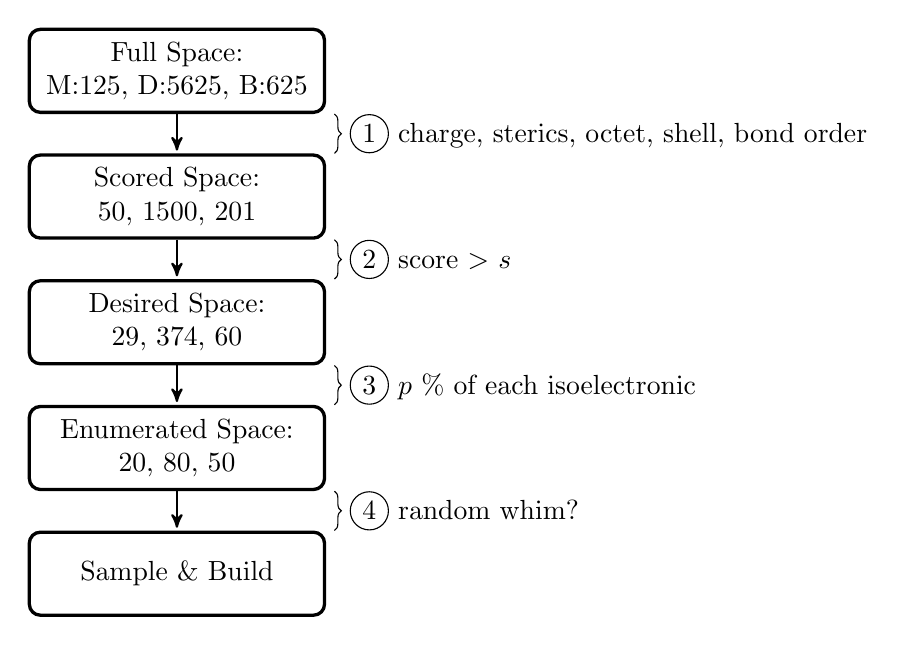
\begin{tikzpicture}
 [node distance=.5cm,
 start chain=going below,]
 \node[punktchain, join] (full) {Full Space: \\ M:125, D:5625, B:625};
 \node[punktchain, join] (scored){Scored Space: \\ 50, 1500, 201};
 \node[punktchain, join] (desi){Desired Space: \\ 29, 374, 60};
 \node[punktchain, join] (enum){Enumerated Space: \\ 20, 80, 50};
 \node[punktchain, join] (sampl){Sample \& Build };
 
 \draw[tuborg, decoration={brace}] let \p1=(full.south), \p2=(scored.north) in
 ($(2, \y1)$) -- ($(2, \y2)$) node[tubnode] {\circled{1} charge, sterics, octet, shell, bond order};
 \draw[tuborg] let \p1=(scored.south), \p2=(desi.north) in
 ($(2, \y1)$) -- ($(2, \y2)$) node[tubnode] {\circled{2} score $>$ $s$};
 \draw[tuborg] let \p1=(desi.south), \p2=(enum.north) in
 ($(2, \y1)$) -- ($(2, \y2)$) node[tubnode] {\circled{3} $p$ \% of each isoelectronic};
 \draw[tuborg] let \p1=(enum.south), \p2=(sampl.north) in
 ($(2, \y1)$) -- ($(2, \y2)$) node[tubnode] {\circled{4} random whim?};
 \end{tikzpicture}
 \caption{A diagram delineating the steps taken to truncate the full space into a space feasible for enumeration. The three numbers under the space label denote the number of mono-heavy-atomic, di-heavy-atomic, and tetra-heavy-atomic bidentate ligands obtained after the reduction step. On the right, the reduction criteria are listed.}
 \label{fig:truncation}
 \end{figure}
 
 \begin{infobox}[Valency (IUPAC Definition)]
 The maximum number of univalent atoms (originally hydrogen or chlorine atoms) that may combine with an atom of the element under consideration, or with a fragment, or for which an atom of this element can be substituted.
 \label{info:valency}
 \end{infobox}
 
% % % % % % % % % % % % % % % % % % %
\subsection{Spanning the full space}
% % % % % % % % % % % % % % % % % % %
For each element CNOPS we allow a charge $c \in \{-2,-1,0,1,2\}$ (we suppress the denticity and atom indices $i$ and $j$ where it is clear from the context) and a number of attached hydrogen atoms $h \in \{0,1,2,3,4\}$.

For the \textbf{MHALs}, we combinatorially cycle through all combinations of elements, of charge, and of number of H atoms, resulting in $5^3=125$ candidates. 

The \textbf{DHALs} were enumerated similarly, iterating through $e_1$, $e_2$, $h_1$, and $h_2$. Since, from a DFT perspective, charge is not a local property, we don't iterate over all combinations of $c_1$ and $c_2$, since it would produce many degeneracies (i.e. $-1+1=0$ is the same overall charge as $-2+2=0$) and it would not be clear, which charge distribution would be the right one, from a classical picture. For that reason, we iterate over a total charge $c_{tot}$. For every instance of $c_{tot}$, we call a subroutine that exhaustively checks all charge combinations that could result in $c_{tot}$. For each combination of charges $c_1$ and $c_2$, we calculate the valency $\nu$ (see Box \ref{info:valency}) of the respective atom as follows, given the lone pairs, $l_i$ and valence electrons $v_i$ from previous knowledge:

\begin{equation}
\label{eq:valency}
\nu_i = v_i - c_i - 2 \cdot l_i - 2 \cdot h_i ~. 
\end{equation}

We set the bond order $b$ to be the minimum of the valencies of the two atoms in the DHAL,

\begin{equation}
b = \min{\{\nu_1,\nu_2\}} ~,
\end{equation}

if the absolute difference of $\nu_1$ and $\nu_2$ is smallest over all charge combinations and $0 \leq b \leq 4$. The optimal charge distribution over the two atoms is assumed to be the $c_1$ and $c_2$ fulfilling the requirements above. If none of these criteria is fulfilled, we set a zero bond order, denoted as $\#0$ in the SMILES formalism. This resulted in 5625 DHALs.

Since the \textbf{THALs} are composed of two bonded DHALs (labeled 1 and 2 for the first DHAL and $1^\prime$ and $2^\prime$ for the second DHAL, 1 and $1^\prime$ being the connecting atom), instead of building them from scratch, we decided to combine all the DHALs and exclude the ones that do not bond effectively. As before, we iterate through $e_1$, $e_2$, $h_1$, and $h_2$ of the building block DHAL. Similarly as with the regular DHAL enumeration described above, we assign a total charge $c_{tot}$ to one of the building block DHALs. We cycle then through all combinations of $c_1$ and $c_2$ and calculate the valencies of each atom according to Eq. (\ref{eq:valency}). If $\nu_1 > 0$, it means that it has at least one electron to bond with atom 2 and if $\nu_2 > 1$, it means that it has at least two electrons, one to bond with atom 1 and one to bond with atom $2^\prime$ of the other DHAL. Since the problem is symmetrical, the valencies $\nu_{1^\prime} > 0$ and $\nu_{2^\prime} > 0$ are exactly the same and only labeled differently to speak about them more effectively. The bond order $b_{12} \in \{1, ..., \nu_2\}$ is chosen as

\begin{equation}
\min_b\{|\nu_2 - \nu_2 - b_{12}|\}
\end{equation}

from which we can simply calculate the second bond, $b_{23}$, as

\begin{equation}
b_{23} = \min\{\nu_1, \nu_2 - b_{12}\} ~.
\end{equation}

We have two possibilities to choose the best charge and bond distribution: Either we require to have minimal bond orders or minimal absolute charges. We decided in favor of minimal charges, since this promises better stability for the resulting complexes. So, if $|c_1|$ and $|c_2|$ are smallest, we choose the corresponding bond orders and charges as the best ones. If none of these criteria is fulfilled, we set a zero bond order, denoted as $\#0$ in the SMILES formalism. This resulted in a total of 5625 THALs.

% % % % % % % % % % % % % % % % % % %
\subsection{The scored and the desired space}
% % % % % % % % % % % % % % % % % % %
In all three sets, we discard open shell compounds, since it leads to difficulties with the DFT calculations.

% % %MHALS
In the set of \textbf{MHALs}, we discard all compounds with a charge outside the boundaries $1 \geq c \geq -3$. We will see this asymmetric restriction towards positive charge throughout this paper, since we know that positive charge usually aggregates on the metal center which leads to instability and negative charges are rather common in ligands. For the remaining compounds, we impose the following scores, $s$, for charges

\begin{equation}
	s_{\textrm{charge}} = 
	\begin{cases}
	0	&	\mathrm{if}~ c = 1 \\
	3	&	\mathrm{if}~ 0 \geq c \geq -2 \\
	0   &	\mathrm{if}~ c = -3 ~,
	\end{cases}
\end{equation}

for the number of H atoms on the connecting atom (CA), which measures sterics,

\begin{equation}
	s_{\textrm{sterics}} = 
	\begin{cases}
	0	&	\mathrm{if}~ h = 4 \\
	3	&	\mathrm{if}~ h \leq 3 ~,
	\end{cases}
\end{equation}

and for the octet rule,

\begin{equation}
	s_{\textrm{octet}} = 
	4 - (|8-v|) ~.
\end{equation}

This leads to a total score,

\begin{equation}
	s = s_{\textrm{charge}} + s_{\textrm{sterics}} + s_{\textrm{octet}} ~.
\end{equation}

A total of 50 compounds were scored, spanning the scored space. From these, we took all with a score $s > 7$ to span the desired space (see Figure \ref{fig:mhalhist}). A 2D histogram of score vs. valence electrons can be seen in Figure \ref{fig:mhal2dhist} In Figure \ref{fig:mhalhist_charge} we can see a distribution of the charges over the desired space of MHALs. No positive charges were selected. 

\begin{figure}[]{}
\centering
\includegraphics[width=.7\linewidth]{img/mhal_ss_hist.pdf} 
\caption{Histogram of all scored MHALs. The ones excluded in the beginning are not shown.}
\label{fig:mhalhist}
\end{figure}

\begin{figure}[]{}
\centering
\includegraphics[width=.7\linewidth]{img/mhal_ss_score_vs_v_2d_hist.pdf} 
\caption{A 2D histogram to show the relationship between score and valence electrons.}
\label{fig:mhal2dhist}
\end{figure}

\begin{figure}[]{}
\centering
\includegraphics[width=.7\linewidth]{img/mhal_ss_hist_charge.pdf} 
\caption{A histogram of the desired MHALs's charges. No positive charges were selected.}
\label{fig:mhalhist_charge}
\end{figure}

% % %DHALS
The \textbf{DHALs} are restricted in a similar way as the MHALs: We discard all compounds with charge $c > 1$ and a number of H atoms on the CA, $h > 3$, since it is not sterically accessible. Lastly, we remove the compounds with a bond order $b = 0$. For the remaining compounds, we impose the following scores, $s$, for polarization

\begin{equation}
	s_{\textrm{polarization}} = 
	\begin{cases}
	0	&	\mathrm{if}~ |c_1| + |c_2| = 4 \\
	1	&	\mathrm{if}~ |c_1| + |c_2| = 3 \\
	3   &	\mathrm{if}~ \mathrm{otherwise} ~,
	\end{cases}
\end{equation}

to punish high polarization between atom 1 and 2. We slightly prefer single bonds over other types of bonds,

\begin{equation}
	s_{\textrm{bond}} = 
	\begin{cases}
	3	&	\mathrm{if}~ b = 1 \\
	2	&	\mathrm{if}~ \textrm{otherwise} ~.
	\end{cases}
\end{equation}

Charge is scored as follows, with $c_{tot} = c_1 + c_2$,

\begin{equation}
u_{\textrm{charge}} = 
\begin{cases}
0	&	\mathrm{if}~ c_{tot} = 1 \\
3	&	\mathrm{if}~ c_{tot} = 0 \\
2   &	\mathrm{if}~ -1 \geq c_{tot} \geq -2 \\
1   &	\mathrm{if}~ c_{tot} = -3 \\
0   &	\mathrm{if}~ c_{tot} = -4 ~,
\end{cases}
\end{equation}

valency as follows,

\begin{equation}
	s_{\textrm{valency}} = 5 - |\nu_1 - \nu_2| ~,
\end{equation}

and the sterics as

\begin{equation}
	s_{\textrm{sterics}} = 
	\begin{cases}
	0	&	\mathrm{if}~ h = 3 \\
	3	&	\mathrm{if}~ h \leq 2 ~.
	\end{cases}
\end{equation}

The total score is then again the sum over all scores,

\begin{equation}
	s = s_{\textrm{polarization}} + s_{\textrm{bond}} + s_{\textrm{charge}} + s_{\textrm{valency}} + s_{\textrm{sterics}} ~.
\end{equation}

In Figure \ref{fig:dhalhist} a histogram of the scores is shown. In total, 1500 compounds were scored, spanning the scored space. If we truncate the space at a score $s > 9$ we can reduce the space to the desired space, which only contains 372 remaining compounds. In Figure \ref{fig:dhalhist} we see a 2D histogram. A trend is visible that a higher score favors more neutral charge. The bond orders decrease the larger they get (see Figure \ref{fig:dhalhist_bo}) and the charge is biased towards neutral (see Figure \ref{fig:dhalhist_charge}).

\begin{figure}
\centering
\begin{overpic}[width=0.8\linewidth]{../meetings/18-03-28-flashtalk/img/distrDiCNOPS.pdf}
	\put (13,24) {[C--]=[OH2--]}
	\put (15,31) {[N--]-[PH4--]}
	\put (25,37) {[CH3]-[SH2-]}
	\put (30,45) {[PH++]\#0[SH3-]}
	
	\put (56,53) {[NH2]-[OH]}
	\put (80,57) {[C+]\#[O-]}
	\put (78,51) {[O-]\#[O-]}
\end{overpic}

\caption{Histogram of all scored DHALs. The ones excluded in the beginning are not shown. Some examples are shown, representing bins at certain scores.}
\label{fig:dhalhist}
\end{figure}

\begin{figure}[]{}
\centering
\includegraphics[width=.7\linewidth]{img/mhal_ss_score_vs_v_2d_hist.pdf} 
\caption{A 2D histogram to show the relationship between score and valence electrons of the DHALs.}
\label{fig:dhal2dhist}
\end{figure}

\begin{figure}[ht] 
	\begin{minipage}[b]{0.5\linewidth}
		\centering
		\includegraphics[width=.9\linewidth]{img/dhal_ss_hist_bo.pdf} 
		\caption{A histogram of the desired DHALs's bond orders. We see that we have much more low bond orders than high bond orders..} 
		\label{fig:dhalhist_bo}
		\vspace{4ex}
	\end{minipage}%%
	\begin{minipage}[b]{0.5\linewidth}
		\centering
		\includegraphics[width=.9\linewidth]{img/dhal_ss_hist_charge.pdf} 
		\caption{A histogram of the desired DHALs's charges. We can observe a bias towards neutral ligands as well as a disfavor of positive ligands.} 
		\vspace{4ex}
		\label{fig:dhalhist_charge}
	\end{minipage}
\end{figure}

% % %THALS
Lastly, we exclude from the scoring all compounds with triple bonds, allenic compounds, and compounds outside the charge range $2 \geq c_{tot} \geq -4$ from the set of \textbf{THALs}.
The bonds are scored with 

\begin{equation}
	s_{\textrm{bond}} = 
	\begin{cases}
	3	&	\mathrm{if}~ b_{12} = b_{12} = 1 \\
	3	&	\mathrm{if}~ b_{23} = 2 \\
	0	&	\mathrm{if}~ b_{12} = 2 ~.
	\end{cases}
\end{equation}

where the double bond in one place determines the other bond to be a single bond. Valency is scored as

\begin{equation}
	s_{\textrm{valency}} = 5 - |\nu_1 - \nu_2| ~,
\end{equation}

sterics on the CA as

\begin{equation}
	s_{\textrm{sterics}} = 
	\begin{cases}
	0	&	\mathrm{if}~ h_1 = 3 \vee h_2 = 3 \\
	3	&	\mathrm{if}~ \textrm{otherwise} ~,
	\end{cases}
\end{equation}

where the $ h_1 = 3 \wedge h_2 = 3 $ case never happens. Finally, the charge is scored as

\begin{equation}
u_{\textrm{charge}} = 
\begin{cases}
5	&	\mathrm{if}~ c_1 = 1 \vee c_2 = 0 \\
3	&	\mathrm{if}~ (c_1 = 1 \vee c_2 = -1) \wedge (c_1 = -1 \vee c_2 = 1) \\
3   &	\mathrm{if}~ (c_1 = -1 \vee c_2 = -1) \\
0   &	\mathrm{if}~ (c_1 = -2 \vee c_2 = -2) \\
3   &	\mathrm{if}~ (c_1 = 0 \vee c_2 = -1) \wedge (c_1 = -1 \vee c_2 = 0) \\
0   &	\mathrm{if}~ (c_1 = 2 \vee c_2 = -1) \wedge (c_1 = -1 \vee c_2 = 2) \\
2   &	\mathrm{if}~ (c_1 = 0 \vee c_2 = -2) \wedge (c_1 = -2 \vee c_2 = 0) \\
1   &	\mathrm{if}~ (c_1 = -2 \vee c_2 = -1) \wedge (c_1 = -1 \vee c_2 = -2) \\
2   &	\mathrm{if}~ (c_1 = -2 \vee c_2 = 0) \wedge (c_1 = 0 \vee c_2 = -2) ~.
\end{cases}
\end{equation}

The total score for the THALs is then the sum over all subtotals:

\begin{equation}
	s =  s_{\textrm{bond}}  + s_{\textrm{valency}} + s_{\textrm{sterics}} + s_{\textrm{charge}} ~.
\end{equation}

In total, 1635 THALs were scored which we reduced to 148 THALs by selecting only the ones with a score higher than $13$. In Figure \ref{fig:thalhist} we see a 2D histogram of charge vs. isoelectronics. The bond orders decrease the larger they get (see Figures \ref{fig:thalhist_b12} and \ref{fig:thalhist_b23}) and the charge is biased towards neutral (see Figures \ref{fig:thalhist_c1}, \ref{fig:thalhist_c2}, and \ref{fig:thalhist_charge}).

\begin{figure}[]{}
\centering
\includegraphics[width=.7\linewidth]{img/thal_ss_hist.pdf} 
\caption{Histogram of all scored THALs. The ones excluded in the beginning are not shown.}
\label{fig:thalhist}
\end{figure}

\begin{figure}[]{}
\centering
\includegraphics[width=.7\linewidth]{img/thal_ss_score_vs_v_2d_hist.pdf} 
\caption{A 2D histogram to show the relationship between score and valence electrons of the THALs.}
\label{fig:thal2dhist}
\end{figure}

\begin{figure}[ht] 
	\begin{minipage}[b]{0.5\linewidth}
		\centering
		\includegraphics[width=.9\linewidth]{img/thal_ss_hist_b12.pdf} 
		\caption{A histogram of the desired THALs's bond orders in bond $b_{12}$. We only see single bonds, as is expected.} 
		\label{fig:thalhist_b12}
		\vspace{4ex}
	\end{minipage}%%
	\begin{minipage}[b]{0.5\linewidth}
		\centering
		\includegraphics[width=.9\linewidth]{img/thal_ss_hist_b23.pdf} 
		\caption{A histogram of the desired THALs's bond orders in bond $b_{23}$. We see a few double bonds, as might be sterically expected.} 
		\vspace{4ex}
		\label{fig:thalhist_b23}
	\end{minipage}
		\begin{minipage}[b]{0.5\linewidth}
			\centering
			\includegraphics[width=.9\linewidth]{img/thal_ss_hist_c1.pdf} 
			\caption{A histogram of the desired THALs's charges on $c_1$. We can observe a bias towards neutral ligands as well as a slight disfavor of positive ligands.} 
			\label{fig:thalhist_c1}
			\vspace{4ex}
		\end{minipage}%%
		\begin{minipage}[b]{0.5\linewidth}
			\centering
			\includegraphics[width=.9\linewidth]{img/thal_ss_hist_c2.pdf} 
			\caption{A histogram of the desired THALs's charges on $c_2$. We can observe a bias towards neutral ligands as well as a slight disfavor of positive ligands.} 
			\vspace{4ex}
			\label{fig:thalhist_c2}
		\end{minipage}
\end{figure}

\begin{figure}[]{}
	\centering	
	\includegraphics[width=.9\linewidth]{img/thal_ss_hist_charge.pdf} 
	\caption{A histogram of the desired THALs's charges on $c_{tot}$. We can observe a bias towards neutral ligands as well as a slight disfavor of positive ligands.} 
	\label{fig:thalhist_charge}
\end{figure}

\subsection{The realm of the possible: The enumerated space}
The enumerated space, $\mathcal{S} \subset \mathbb{R}^{155}$, will be the space in which our solutions live, accounting for the 155 RACs. Our constraints allow us to assemble around 1.5~M complexes. We choose 20 MHALs, 80 DHALs and 50 THALs. Constraining on weak symmetry (axial positions distinguishable, symmetrical equatorial positions), we obtain $(20 + 80)^3 + 50^2 + 50 \cdot 100^2 = 1,502,500$ compounds. 

The 20 MHALs were chosen uniformly proportionally to their isoelectronic distribution, around 66~\% of each bin of isoelectronics. The DHALs were chosen accordingly, around 20~\% of each bin. The bidentates were chosen without regard on the isoelectronic distribution.

\newpage 
\section{Ligand Field Assembly}

\subsection{Subsets of octahedral space}
The full combinatorial space of all ligands generated in Section \ref{sec:enum} is vast with a lower estimated bound of $> 1.8 \cdot 10^{14}$, calculated from cube coloring theorem. The difficulty is to include bidentate symmetry into the calculations. In the following, we will motivate why only a fraction of the full space is of interest. This will give us the possibility of actually enumerating the ligand fields and calculate properties of the subsets.
One goal of this work is to be able to fine tune molecular properties such as oxidation energy or spin splitting energy. It seems natural to assume that a full set of all possible ligand fields gives the most fine grained raster over all possible properties, a complex could have. This might be statistically true but also prevent rigorous analysis. The set is too dense to traverse on a computationally feasible time scale. We propose the homoleptic subset of the octahedral space as a backbone. Conceptually, homoleptic octahedral compounds must be on the edge of the actual octahedral space, since the properties of single complexes do not get more distinct than in homoleptic ones. From the homoleptic complex space it is possible to go to lower symmetry classes and get closer to a complex with desired properties without analyzing all complexes on the way. This reduces computational cost by several orders of magnitude. Our selection of complexes can be found in Table \ref{tab:space-sizes}. They were chosen to be of highest possible symmetry to result in the smallest number of complexes and to be synthetically interesting. 
\begin{table}[]
	\centering
	\caption{The sizes of the selected subsets of octahedral space.}
	\label{tab:space-sizes}
	\begin{tabular}{llr}
		\toprule
		Set 					& description		    	   & size \\
		\midrule
		Homoleptics             & eq = ax                   & 553        \\[0.1cm]
		"5+1" symmetric         & eq = ax1 $\neq$ ax2       & 163,620    \\[0.1cm]
		"4+2" symmetric         & eq1 $\neq$ eq2 = ax       & 185,376    \\[0.1cm]
		Strongly symmetric      & eq $\neq$ ax              & 245,316    \\[0.1cm]
		Equatorially asymmetric & eq1 $\neq$ eq2 $\neq$ ax  & 15,924,796 \\[0.1cm]
		Weakly symmetric        & eq $\neq$ ax1 $\neq$ ax2  & 45,077,310 \\[0.1cm]
		Complete Heteroleptics  & $L_i \neq L_j$            & $\approx 5.9 \cdot 10^{12}$ \\[0.1cm] %405!/399!/6!+148!/145!/3!
		Octahedral Space        & all                       & $> 1.8 \cdot 10^{14}$ \\
		%number of cube colorings as lower bound
		\bottomrule
	\end{tabular}
\end{table}




%\subsection{Properties of the sets}
%\begin{itemize}
%\item Reduce space to facilitate sampling from non-homoleptics
%\item Example: strongly symmetric, monodentate ligand fields (163,620)
%\item Exclude all with charge smaller than -4, which results in 87,150 ligand fields (53~\%).
%\end{itemize}
%\begin{figure}[ht] 
%	\begin{minipage}[b]{0.5\linewidth}
%		\centering
%		\includegraphics[width=.8\linewidth]{img/strongsymMonodentates_chargeHist.pdf} 
%		\vspace{4ex}
%	\end{minipage}%%
%	\begin{minipage}[b]{0.5\linewidth}
%		\centering
%		\includegraphics[width=.8\linewidth]{img/strongsymMonodentates_chargeHistCum.pdf} 
%		\vspace{4ex}
%	\end{minipage} 
%\end{figure}

\subsection{Subset analysis}
We did a principal component analysis on the homoleptic subspace and projected the strongly symmetric and "5+1" symmetric subspace onto it (see Figure \ref{fig:pca}). The connecting atom is colored according to the CPK coloring with a gradient transition from oxygen (red) to phosphorus(orange). The connecting atom is the average over all 6 connecting atoms. We can see that the gap on PC2 separates first period elements from second order elements in the homoleptic case. Going to lower symmetry, we see that this gap is filled up with fractional element types. This sonsolidates our hypothesis that the homoleptics build the backbone of the full space and that lowering symmetry allows us to find more fine grained complexes.

\begin{figure}
\includegraphics[width=0.7\linewidth]{img/pca.pdf}
\centering
\caption{A PCA on the homoleptic subspace. The strongly symmetric (ss) and "5+1" symmetric (fo) subspace were projected onto it. The connecting atom identity (cai) is encoded in the color following CPK coloring with a gradient transition from oxygen (red) to phosphorus (orange).}
\label{fig:pca} 
\end{figure}

\subsection{Entropy of the subsets}
To compare the different subsets, we devised a non-unqiue footprint to characterize the ligand fields in 5 dimensions:
\begin{itemize}
\item total charge
\item total valence electrons
\item electronegativity of the connecting atom
\item $^{\textrm{lc}}_{\textrm{ax,eq}}\chi_1 = \sum{EN_{\textrm{CA}} \cdot EN_i}$
\item $^{\textrm{lc}}_{\textrm{ax,eq}}\chi^\prime_1 = \sum{EN_{\textrm{CA}} - EN_i}$
\end{itemize}

We then calculate the entropy, $H_{\textrm{KDE}}$, of the Kernel Density Estimated (KDE) distrbution and Scott's rule to estimate the bandwidth of the KDE:





%\frametitle{Correlation analysis for strongly symmetric monodentates }
%\begin{figure}
%\includegraphics[width=0.65\linewidth]{img/strongsymMonodentates_PairwiseCorr.png}
%\end{figure}
%\end{frame}
%
%\begin{frame}
%\frametitle{Example of KDE slice}
%Dimensions $^{\textrm{lc}}_{\textrm{ax,eq}}\chi_1$ vs. charge in $H_{\textrm{KDE}}$ for strongly symmetric monodentates.
%\begin{figure}[ht] 
%	\begin{minipage}[b]{0.5\linewidth}
%		\centering
%		\includegraphics[width=1\linewidth]{img/strongsymMonodentates_heatmap.pdf} 
%		\vspace{2ex}
%	\end{minipage}%%
%	\begin{minipage}[b]{0.5\linewidth}
%		\centering
%		\includegraphics[width=1\linewidth]{img/strongsymMonodentates_3Dhists.pdf} 
%		\vspace{2ex}
%	\end{minipage} 
%\end{figure}
%\end{frame}
%
%\begin{frame}
%\frametitle{Monodentate Footprints}
%	\begin{table}[]
%	\centering
%	\caption{Entropic footprint}
%	\label{tab:ent-footprint}
%	\begin{tabular}{lcr}
%		\toprule
%		Set 					    &  $H_{\textrm{KDE}}^{\textrm{monodent}}$   & $H_{\textrm{KDE}}^{\textrm{bident}}$ \\
%		\midrule
%		Homoleptics                 &  19.7  & 15.63   \\[0.1cm]
%		"5+1" symmetric             &  13.7  & -       \\[0.1cm]
%		Strongly symmetric AC       &  -     & 9.47    \\[0.1cm]
%		Strongly symmetric ADC      &  12.70 & 5.53    \\[0.1cm]
%		"4+2" symmetric             &  12.70 & 9.47    \\[0.1cm] 
%		Weakly symmetric            &  8.1   & 7.7     \\[0.1cm]
%		Equatorially asymmetric AC  &  -     & 10.04   \\[0.1cm]
%		Equatorially asymmetric ADC &        &         \\[0.1cm]
%
%		\bottomrule
%	\end{tabular}
%	\end{table}
%\end{frame}
%
%\begin{frame}
%\frametitle{Entropy histogram}
%\begin{figure}
%\includegraphics[width=0.7\linewidth]{img/ent.pdf}
%\end{figure}
%\end{frame}
%
%%
%%\begin{frame}
%%\frametitle{Actual calculations}
%%The calculations, colored by convergence fitness.
%%\begin{figure}
%%\includegraphics[width=0.7\linewidth]{img/pcaWithCalcs.pdf}
%%\end{figure}
%%\end{frame}
%
%\begin{frame}
%\frametitle{Actual calculations}
%\begin{figure}[ht] 
%	\label{ fig7} 
%	\begin{minipage}[b]{0.5\linewidth}
%		\centering
%		\includegraphics[width=.6\linewidth]{img/pcaWithCalcs.pdf} 
%%		\vspace{8ex}
%	\end{minipage}%%
%	\begin{minipage}[b]{0.5\linewidth}
%		\centering
%		\includegraphics[width=.6\linewidth]{img/fateByCharge.pdf} 
%%		\vspace{8ex}
%	\end{minipage} 
%	\begin{minipage}[b]{0.5\linewidth}
%		\centering
%		\includegraphics[width=.6\linewidth]{img/fateBytype.pdf} 
%%		\vspace{4ex}
%	\end{minipage}%% 
%	\begin{minipage}[b]{0.5\linewidth}
%		\centering
%		\includegraphics[width=.6\linewidth]{img/timeByfate.pdf} 
%%		\vspace{4ex}
%	\end{minipage} 
%\end{figure}
%\end{frame}
%
%
%\begin{frame}
%\begin{itemize}
%\item 0: [NH3], [N]\#[N], [C+]\#[O-], [C+]\#[NH-], [N]#[CH]
%\item 1: [CH+]=[CH3-], [NH]=[O], [CH+]=[OH-], [CH2+]-[OH2-]
%\item 8: [OH2-]-[PH+], [P+]=[OH-], [PH+]-[OH2-], [NH2-]=[CH+]
%
%\end{itemize}
%\end{frame}


\end{document}
